% Created 2023-03-11 Sat 20:18
% Intended LaTeX compiler: pdflatex
\documentclass[final, 12pt] {ubb_dolgozat}{book}
\usepackage[utf8]{inputenc}
\usepackage[T1]{fontenc}
\usepackage{graphicx}
\usepackage{longtable}
\usepackage{wrapfig}
\usepackage{rotating}
\usepackage[normalem]{ulem}
\usepackage{amsmath}
\usepackage{amssymb}
\usepackage{capt-of}
\usepackage{hyperref}
\usepackage{minted}
\submityear{2022}
\doctypeHU{Szakdolgozat}
\doctypeEN{Diploma Thesis}
\doctypeRO{Lucrare de licenta}
\specHU{Informatika}
\specEN{Computer Science}
\specRO{Informatică}
\titleHU{Szakdolgozat cím}
\titleEN{License thesis title}
\titleRO{Titlu lucrare licență}
\authorHU{Zediu Álmos-Ágoston}
\authorRO{Álmos-Ágoston Zediu}
\authorEN{Álmos-Ágoston Zediu}
\tutorHU{dr. Bodó Zalán}
\tutorRO{dr. Bodó Zalán}
\tutorEN{dr. Bodó Zalán}
\pagenumbering{gobble}
\author{Álmos-Ágoston Zediu}
\date{\today}
\title{Szakdolgozat}
\hypersetup{
 pdfauthor={Álmos-Ágoston Zediu},
 pdftitle={Szakdolgozat},
 pdfkeywords={},
 pdfsubject={},
 pdfcreator={Emacs 28.2 (Org mode 9.6)}, 
 pdflang={English}}
\usepackage{natbib}
\begin{document}

\maketitle
\tableofcontents


\chapter{Bevezetés}
\label{sec:org5136892}
\chapter{Clojure}
\label{sec:org8c47bb4}
A Clojure programozási nyelv egy dinamikus funkcionális nyelv, mely ötvözi a JVM platform előnyeit a Lisp nyelvek
kifejezőkészségével.
\section{Funkcionális programozás Clojureben}
\label{sec:org15d5cf3}

A Clojureben a függvények az elsőrendű absztrakciók, képesek vagyunk akár argumentumként is kezelni őket, stb.

\begin{minted}[]{clojure}
(defn my-adder [a b]
  (+ a b))

(def my-five-adder (partial my-adder 5))
(map my-five-adder [1, 2, 3, 4])
\end{minted}

\begin{itemize}
\item (``\#'user/my-adder'')
\item (``\#'user/my-five-adder'')
\item (``(6 7 8 9)'')
\end{itemize}

\section{Perzisztens adatstruktúrák}
\label{sec:org164b5cb}
Rich Hickey az adatstruktúráit az ideális hasítófákra alapozta \citep{bagwellIdealHashTrees2001}. Egy konceptuális elképzelésért
rátekinthetünk erre a képre:

\begin{center}
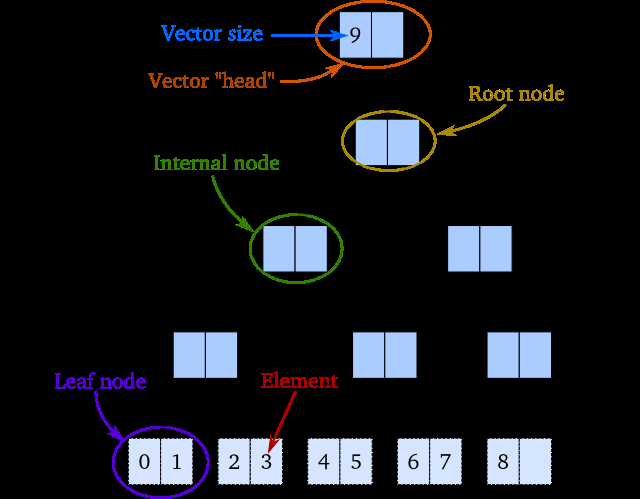
\includegraphics[width=.9\linewidth]{images/perzisztens-vektor.jpg}
\end{center}

A lényegi rész az, hogy ahhoz, hogy olyan adatstruktúrák, mint a vektorok performánsak legyenek, de perzisztensek, szükségünk van
specializált bináris fák felépítésére.

\section{Homoikonicitás}
\label{sec:orgc57cbe3}
Ami talán leginkább megkülönbözteti a Lisp nyelvcsaládban levő nyelveket a többiektől, az a  homoikonicitás \citep{mcilroyMacroInstructionExtensions1960} tulajdonság, vagyis maga a programkód
formálható ugyanazzal a nyelvvel futás közben, mint amiben meg volt írva.

Hasonló viselkedést elérhetünk nem homoikonikus nyelvekben is, mint mondjuk a Java vagy a C\# reflection rendszere, vagy
pedig a Python dekorátor szintaxisa, viszont a Lisp nyelvek makrórendszereivel azért könnyebb valamilyen szinten dolgozni, mivel nincsenek speciálisan megkülönböztetve a programban
felhasznált adatstruktúrák szintaxisai, és a programot felépítő, elágazásokat, ismétlő ciklusokat, függvénydefiníciókat jelző nyelvi struktúrák szintaxisai.

Vegyük példának okáért a következő egyszerű programot:

\begin{minted}[]{clojure}
(defn add-list-numbers [number-list]
  (apply + number-list))

(add-list-numbers '(1 2 3 4 5))
\end{minted}

\begin{itemize}
\item (``\#'user/add-list-numbers'')
\item (``15'')
\end{itemize}

Látható, hogy a függvénydefiníció kerek zárójelekbe írtuk, a függvény argumentumai pedig egy vektorszerű struktúrában kaptak helyet, utána pedig maga a függvényhívás is zárójelek között volt. Érdekes módon az átadott lista szintúgy zárójelezve adódott át, viszont raktunk elé egy aposztrófot is.

Erre azért volt szükség, mivel a Lisp nyelvekben a kerek zárójel listát jelöl, és minden lista, hacsak nem jelezzük aposztróffal, függvénymeghívással jár. Annak köszönhetően viszont, hogy ``listákban'' programozunk, képesek vagyunk a programrészleteinket mint lista, vektor, vagy halmazelemeket
módosítani átrendezni.

\subsection{Makrók}
\label{sec:org3fb8753}
A Lisp makrók olyan programszerkezetek, amelyek egy programrészletet kapnak meg, módosítják azt, és a módosított programrészlet eredményét futtatják végül le. Fontos megjegyezni, hogy ez fordítási időben történik, nem futási időben.

\begin{enumerate}
\item {\bfseries\sffamily TODO} Ezt még átfogalmazni picit
\label{sec:org91f5f97}
Egy jó példa arra, hogyan segíthet ez fejlesztésben és talán még fontosabb, adatelemzés során, az az úgynevezett ``threading'' makró.

\begin{minted}[]{clojure}
(defn generate-masked-grouped-ratings [dataset-path]
  (-> (load-ratings dataset-path)
      (tc/dataset)
      (tc/complete :user :item)
      (tc/group-by :user {:result-type :as-seq})))
\end{minted}

Ez a makró be van építve a nyelvbe, és forráskódja is rövid.

\begin{minted}[]{clojure}
(defmacro ->
  [x & forms]
  (loop [x x, forms forms]
    (if forms
      (let [form (first forms)
            threaded (if (seq? form)
                       (with-meta `(~(first form) ~x ~@(next form)) (meta form))
                       (list form x))]
        (recur threaded (next forms)))
      x)))
\end{minted}
\end{enumerate}

\chapter{Algoritmusok}
\label{sec:org92a14c3}
\section{Locality sensitive hashing}
\label{sec:orge4d1368}
Lehet beszélni erről a \citep{charikarSimilarityEstimationTechniques}, vagy pedig,

\section{SVD}
\label{sec:org27215df}
\citep{brandFastOnlineSVD2003}

\bibliographystyle{./abbrvnat_hu.bst}
\bibliography{/home/hrothgar32/Documents/Egyetem/Allamvizsga/Dolgozat/allamvizsga,/home/hrothgar32/Documents/allamvizsga/allamvizsga}
\end{document}